\chapter{Results and Discussion}

The first set of experiments used the 'toy' artificial data set. \bigskip

The second set of experiments used the MNIST data set. In principle, any modern iteration of a \gls{cnn} can achieve very high accuracy on this data set \cite{sota_web}. \gls{nn}s ranging from simple CNNs to modern CapsNets, \gls{resnet}s and DenseNets (all \gls{dnn}s) should be able to achieve 98-99\% on this data set {\cite{mnist_sota_web}}. This is seen in the test and training accuracies in the baseline training schemes (figure \ref{fig:training_scheme_10_11}), where very high accuracies are achieved after only a few \gls{epoch}s. 
\bigskip

% https://tex.stackexchange.com/questions/140833/arranging-multiple-plots-in-a-grid-inside-a-figure-subfloat

\begin{figure}[H]
    \centering
    \subfloat[first]{
      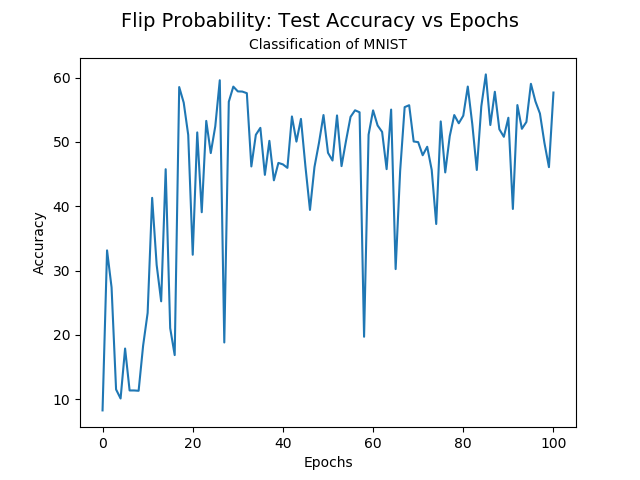
\includegraphics[width=65mm]{figs/run_1/test_accuracy_fp.png}
    }
    \subfloat[second]{
      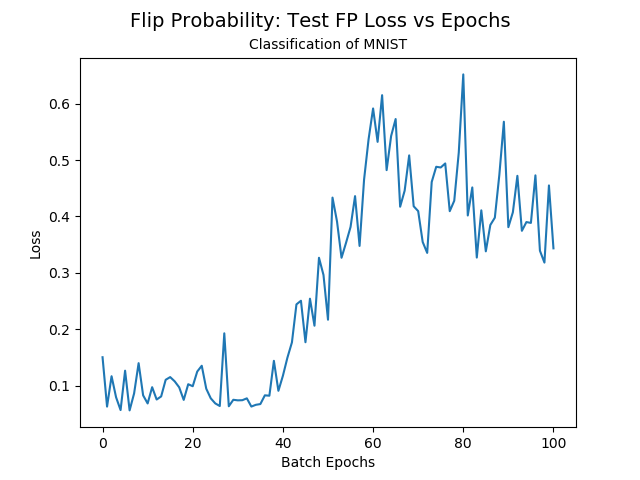
\includegraphics[width=65mm]{figs/run_1/test_losses_fp.png}
    }
    \hspace{0mm}
    \subfloat[third]{
      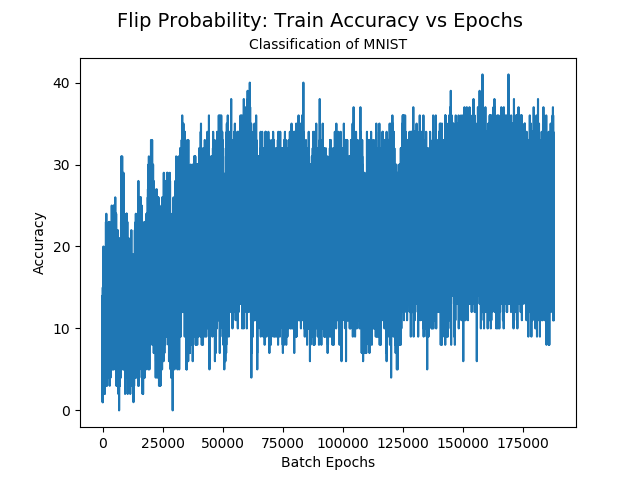
\includegraphics[width=65mm]{figs/run_1/train_accuracy.png}
    }
    \subfloat[forth]{
      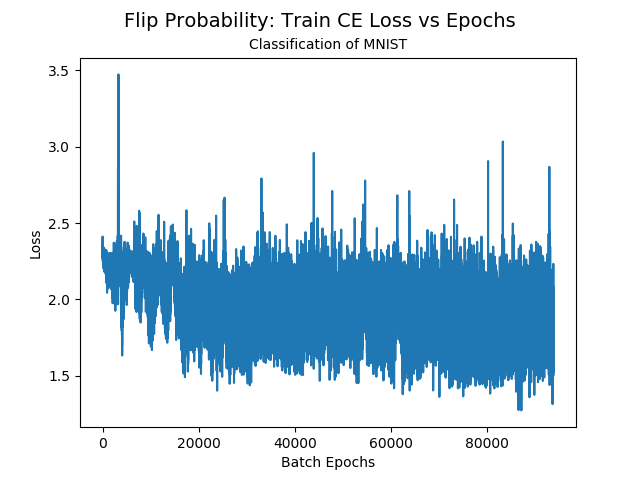
\includegraphics[width=65mm]{figs/run_1/train_losses_ce.png}
    }
    \hspace{0mm}
    \hbox to 67.5mm{}% !!
    \subfloat[fifth]{   % ???
      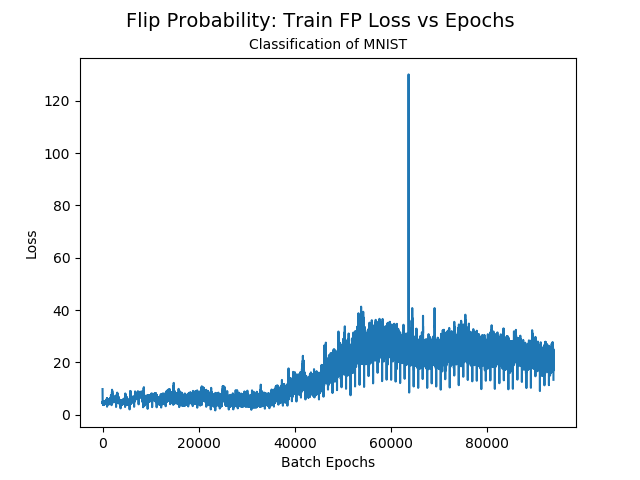
\includegraphics[width=65mm]{figs/run_1/train_losses_fp.png}
    }
    \caption{The results of the initial training scheme}
    \label{fig:training_scheme_1}
    \end{figure}
    
    \begin{figure}
    \centering
    \subfloat[first]{
      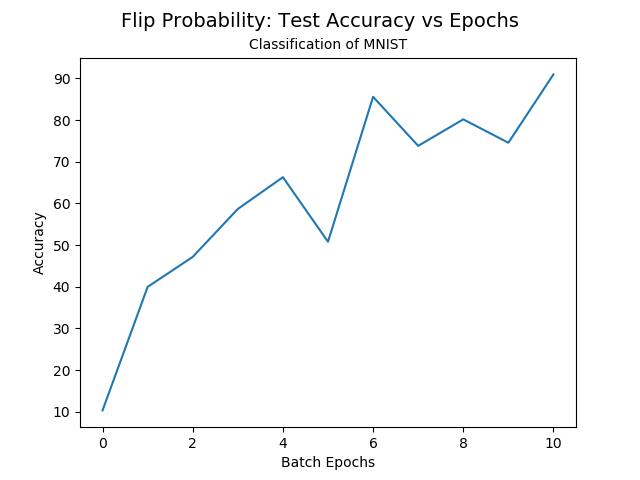
\includegraphics[width=65mm]{figs/run_2/test_accuracy_fp.png}
    }
    \subfloat[second]{
      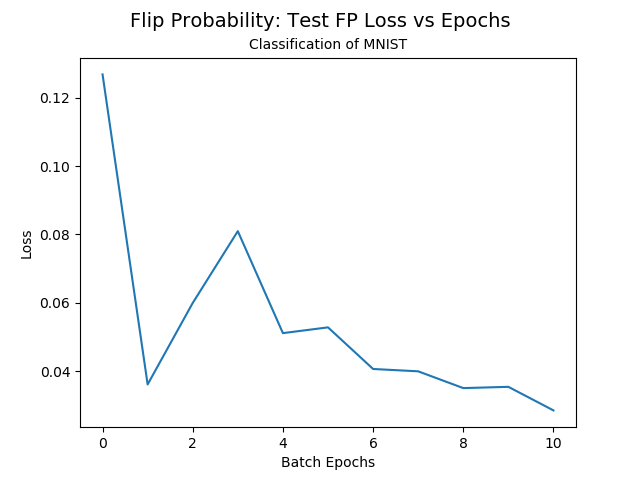
\includegraphics[width=65mm]{figs/run_2/test_losses_fp.png}
    }
    \hspace{0mm}
    \subfloat[third]{
      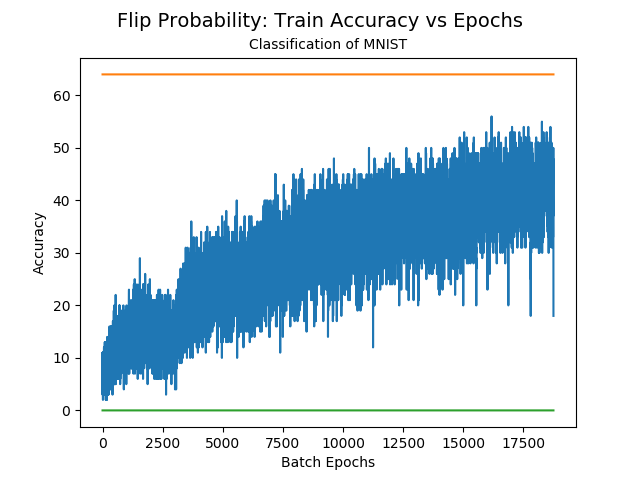
\includegraphics[width=65mm]{figs/run_2/train_accuracy.png}
    }
    \subfloat[forth]{
      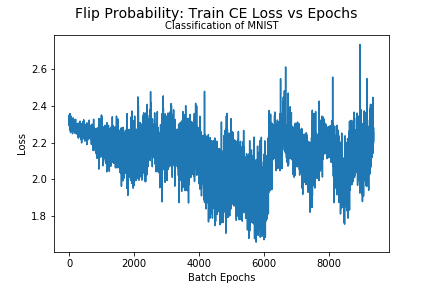
\includegraphics[width=65mm]{figs/run_2/train_losses_ce.png}
    }
    \hspace{0mm}
    \hbox to 67.5mm{}% !!
    \subfloat[fifth]{   % ???
      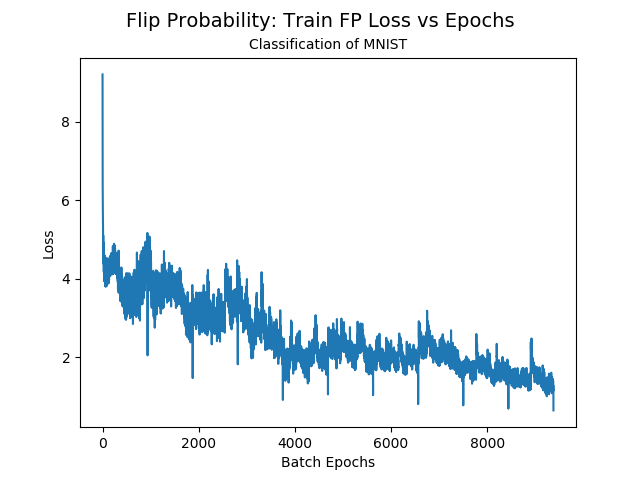
\includegraphics[width=65mm]{figs/run_2/train_losses_fp.png}
    }
    \caption{The results of the second training scheme}
    \label{fig:training_scheme_2}

\end{figure}

\begin{figure}[H]
    \centering
    \subfloat[first]{
      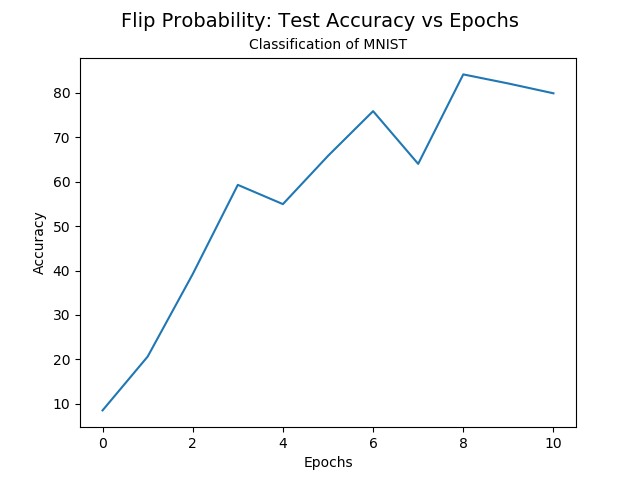
\includegraphics[width=65mm]{figs/run_3/test_accuracy_fp.png}
    }
    \subfloat[second]{
      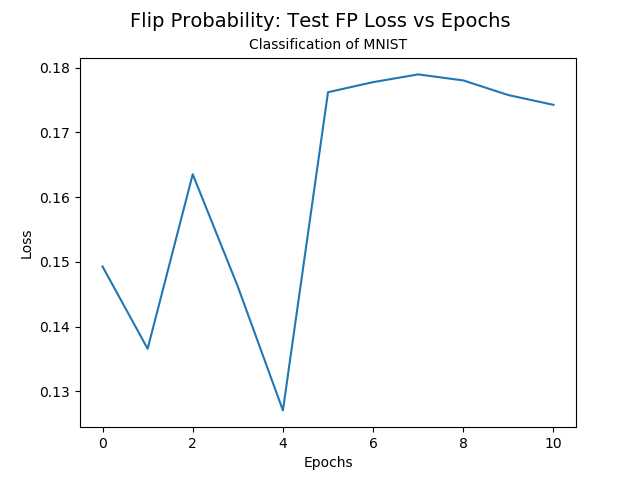
\includegraphics[width=65mm]{figs/run_3/test_losses_fp.png}
    }
    \hspace{0mm}
    \subfloat[third]{
      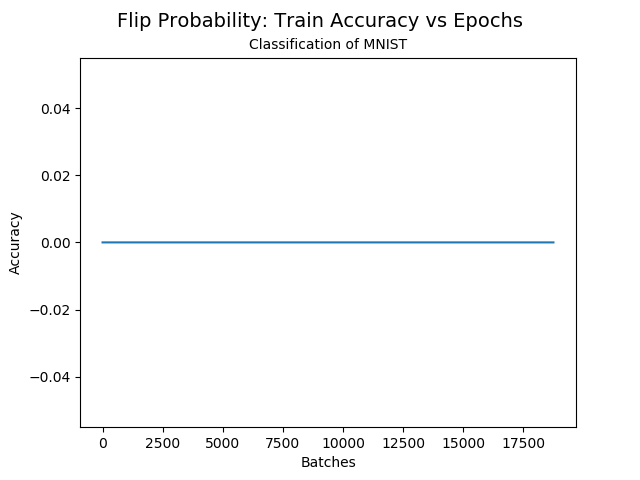
\includegraphics[width=65mm]{figs/run_3/train_accuracy.png}
    }
    \subfloat[forth]{
      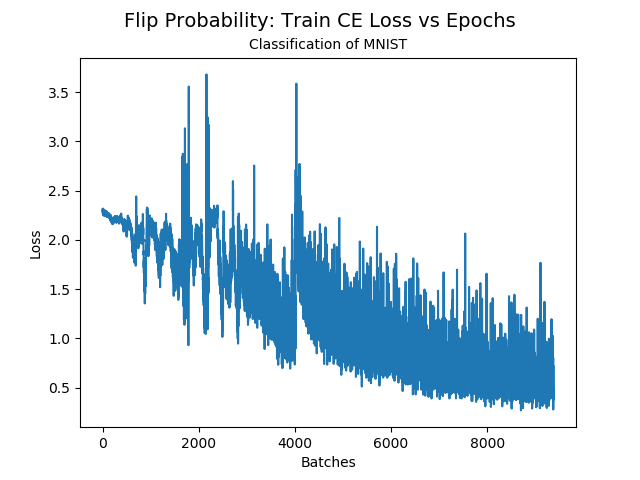
\includegraphics[width=65mm]{figs/run_3/train_losses_ce.png}
    }
    \hspace{0mm}
    \hbox to 67.5mm{}% !!
    \subfloat[fifth]{   % ???
      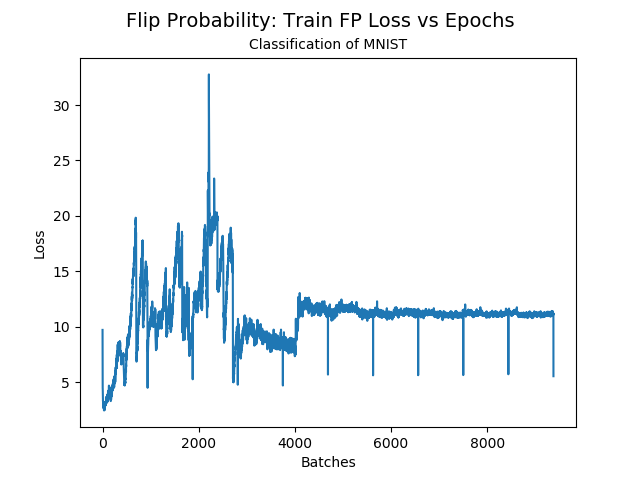
\includegraphics[width=65mm]{figs/run_3/train_losses_fp.png}
    }
    \caption{The results of the third training scheme}
    \label{fig:training_scheme_3}
\end{figure}

\begin{figure}[H]
    \centering
    \subfloat[first]{
      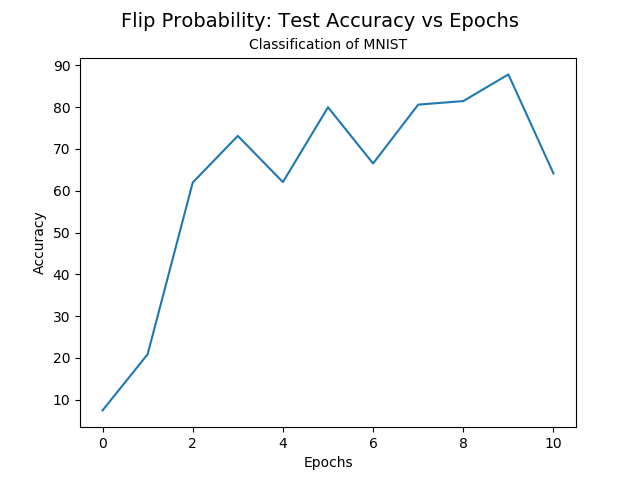
\includegraphics[width=65mm]{figs/run_4/test_accuracy_fp.png}
    }
    \subfloat[second]{
      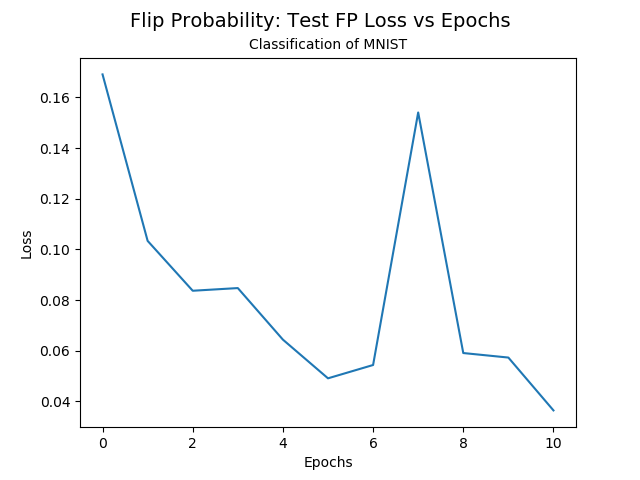
\includegraphics[width=65mm]{figs/run_4/test_losses_fp.png}
    }
    \hspace{0mm}
    \subfloat[third]{
      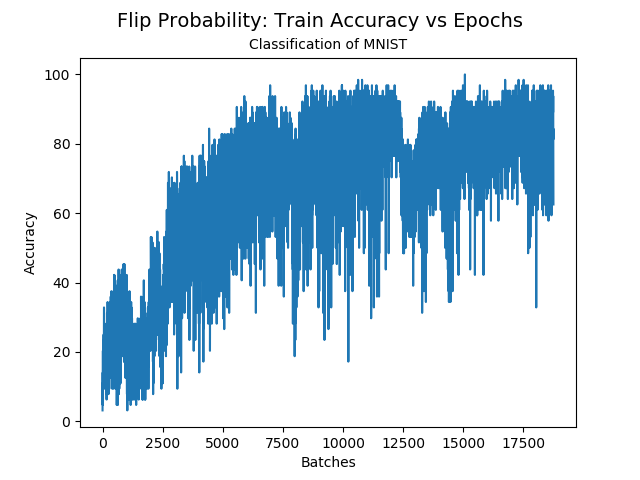
\includegraphics[width=65mm]{figs/run_4/train_accuracy.png}
    }
    \subfloat[forth]{
      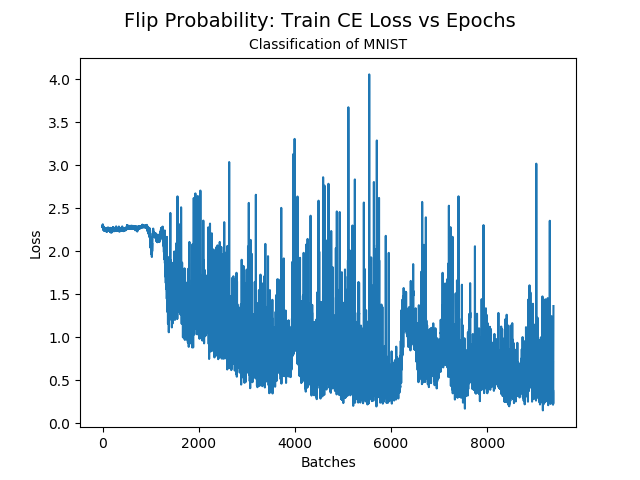
\includegraphics[width=65mm]{figs/run_4/train_losses_ce.png}
    }
    \hspace{0mm}
    \hbox to 67.5mm{}% !!
    \subfloat[fifth]{   % ???
      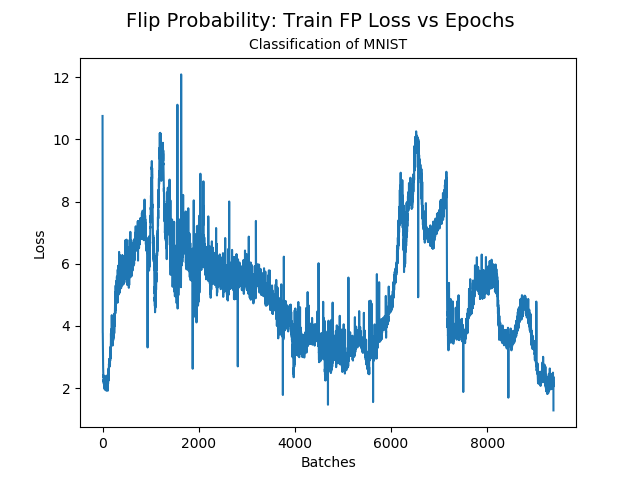
\includegraphics[width=65mm]{figs/run_4/train_losses_fp.png}
    }
    \caption{The results of the fourth training scheme}
    \label{fig:training_scheme_4}
\end{figure}

\begin{figure}[H]
    \centering
    \subfloat[first]{
      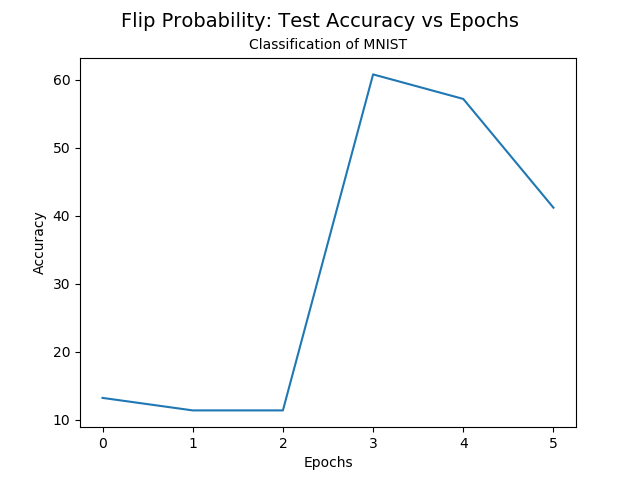
\includegraphics[width=65mm]{figs/run_5/test_accuracy_fp.png}
    }
    \subfloat[second]{
      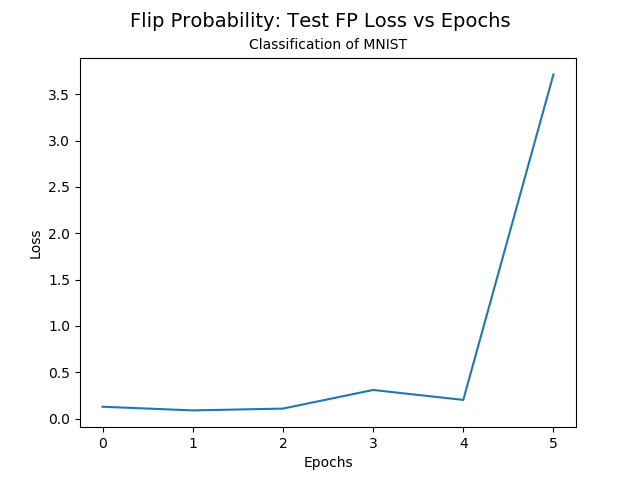
\includegraphics[width=65mm]{figs/run_5/test_losses_fp.png}
    }
    \hspace{0mm}
    \subfloat[third]{
      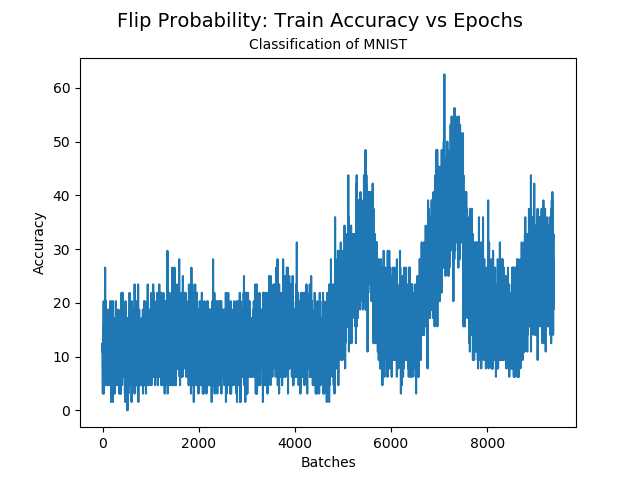
\includegraphics[width=65mm]{figs/run_5/train_accuracy.png}
    }
    \subfloat[forth]{
      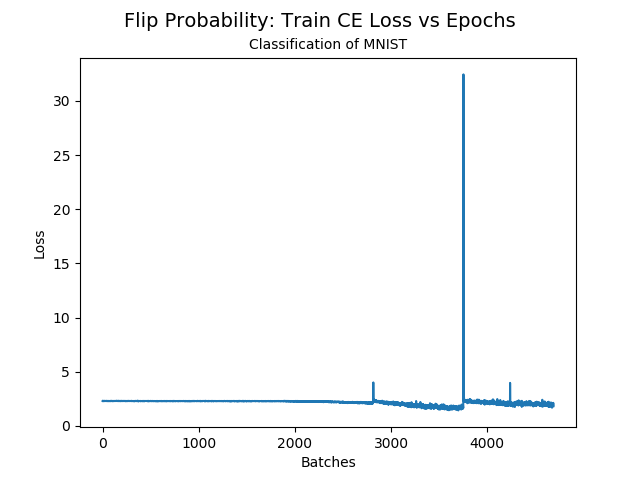
\includegraphics[width=65mm]{figs/run_5/train_losses_ce.png}
    }
    \hspace{0mm}
    \hbox to 67.5mm{}% !!
    \subfloat[fifth]{   % ???
      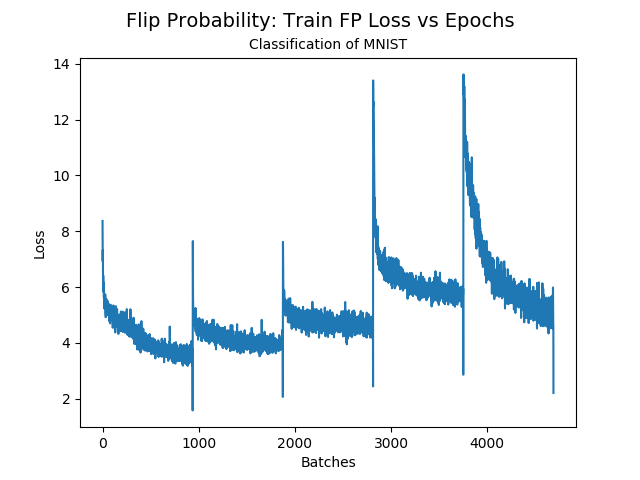
\includegraphics[width=65mm]{figs/run_5/train_losses_fp.png}
    }
    \caption{The results of the fifth training scheme}
    \label{fig:training_scheme_5}
\end{figure}

\begin{figure}[H]
    \centering
    \subfloat[first]{
      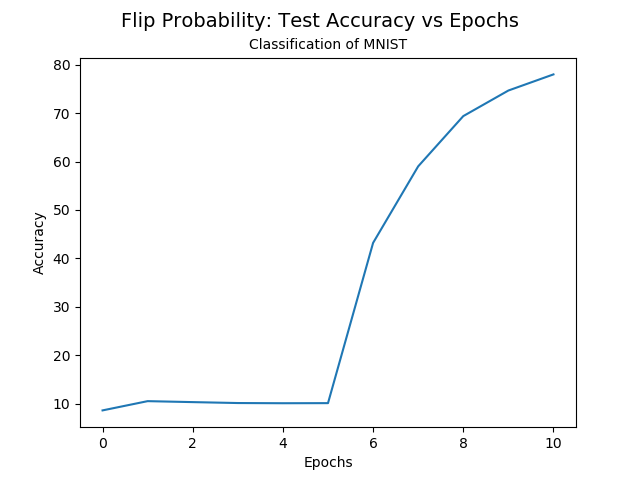
\includegraphics[width=65mm]{figs/run_6/test_accuracy_fp.png}
    }
    \subfloat[second]{
      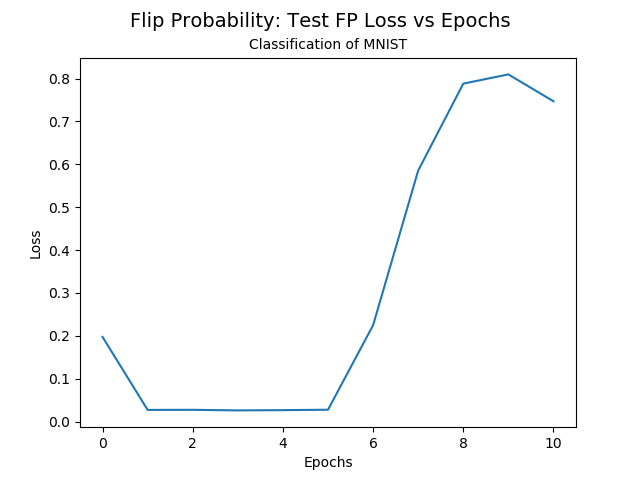
\includegraphics[width=65mm]{figs/run_6/test_losses_fp.png}
    }
    \hspace{0mm}
    \subfloat[third]{
      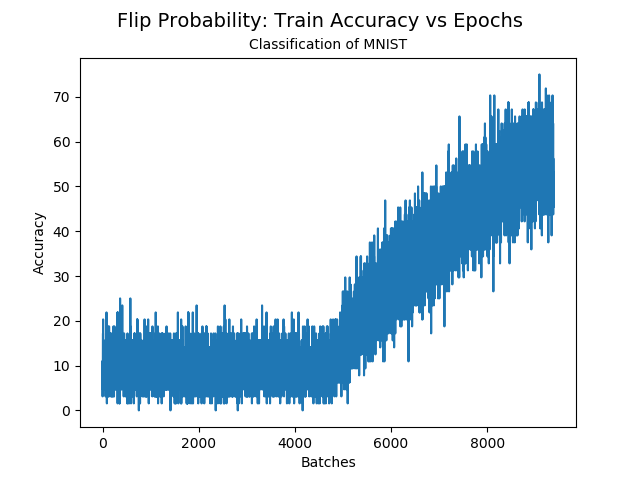
\includegraphics[width=65mm]{figs/run_6/train_accuracy.png}
    }
    \subfloat[forth]{
      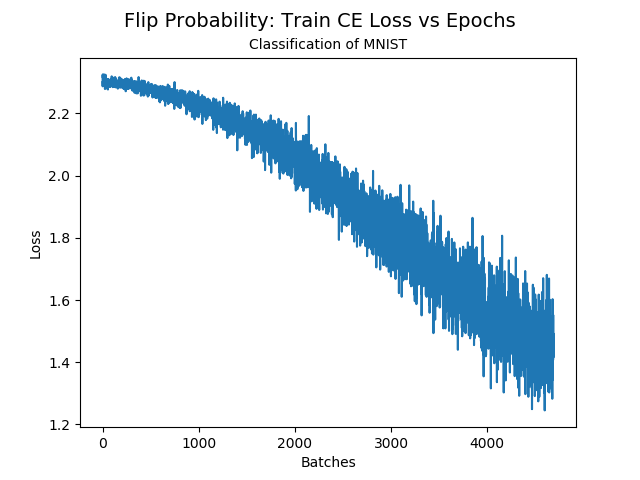
\includegraphics[width=65mm]{figs/run_6/train_losses_ce.png}
    }
    \hspace{0mm}
    \hbox to 67.5mm{}% !!
    \subfloat[fifth]{   % ???
      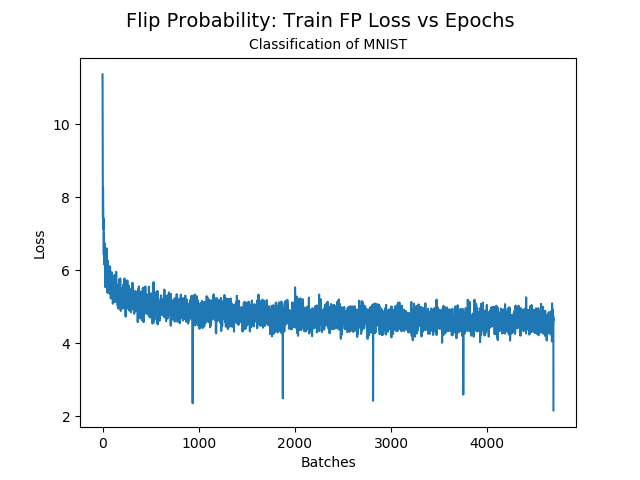
\includegraphics[width=65mm]{figs/run_6/train_losses_fp.png}
    }
    \caption{The results of the sixth training scheme}
    \label{fig:training_scheme_6}
\end{figure}

\begin{figure}[H]
    \centering
    \subfloat[first]{
      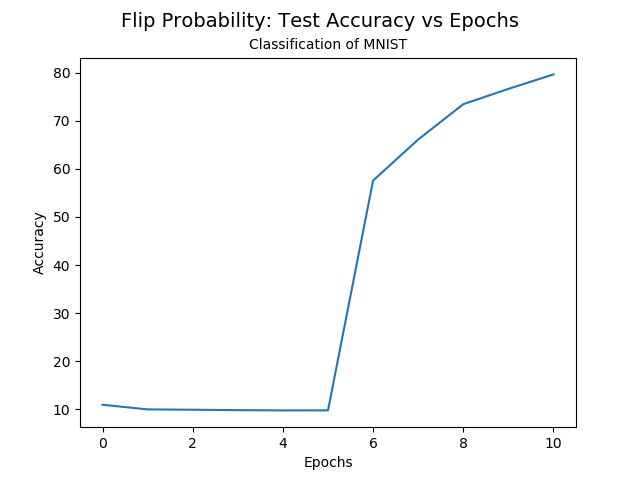
\includegraphics[width=65mm]{figs/run_7/test_accuracy_fp.png}
    }
    \subfloat[second]{
      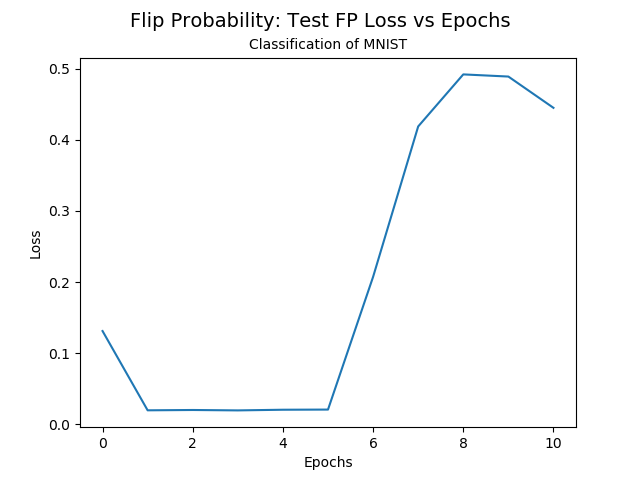
\includegraphics[width=65mm]{figs/run_7/test_losses_fp.png}
    }
    \hspace{0mm}
    \subfloat[third]{
      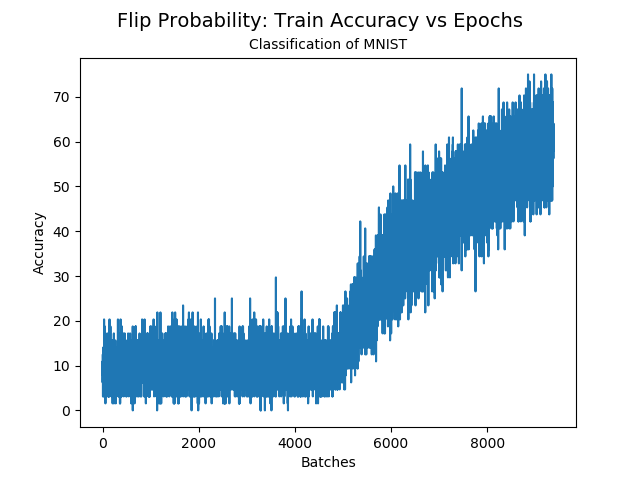
\includegraphics[width=65mm]{figs/run_7/train_accuracy.png}
    }
    \subfloat[forth]{
      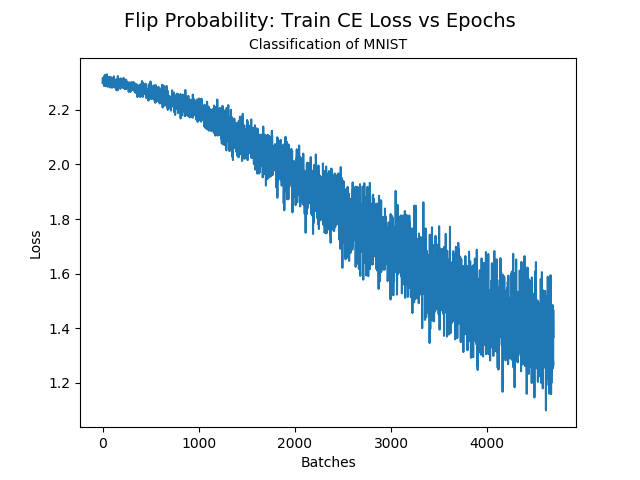
\includegraphics[width=65mm]{figs/run_7/train_losses_ce.png}
    }
    \hspace{0mm}
    \hbox to 67.5mm{}% !!
    \subfloat[fifth]{   % ???
      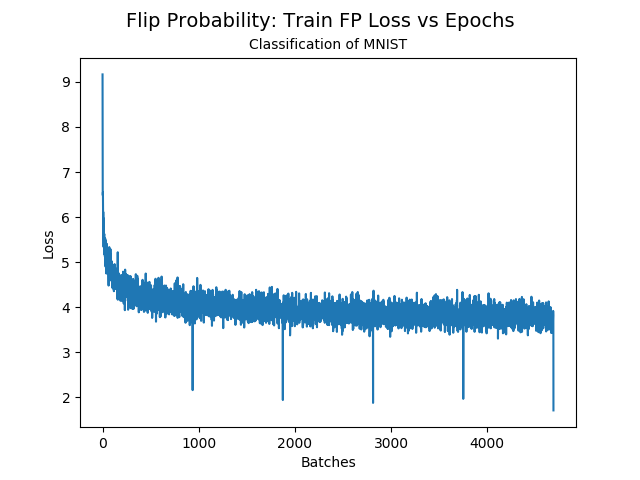
\includegraphics[width=65mm]{figs/run_7/train_losses_fp.png}
    }
    \caption{The results of the seventh training scheme}
    \label{fig:training_scheme_7}
\end{figure}

\begin{figure}[H]
    \centering
    \subfloat[first]{
      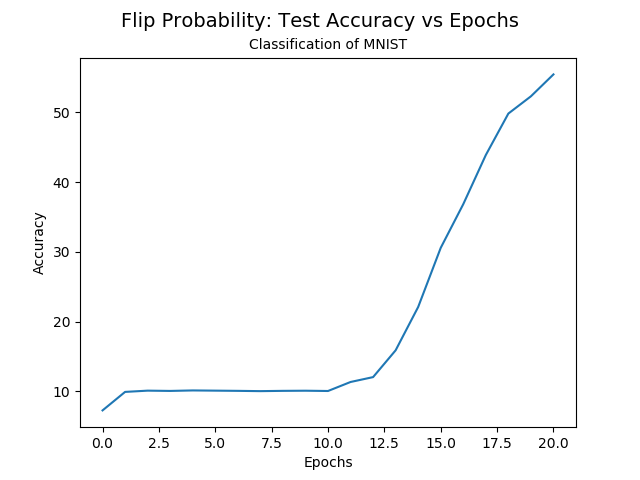
\includegraphics[width=65mm]{figs/run_8/test_accuracy_fp.png}
    }
    \subfloat[second]{
      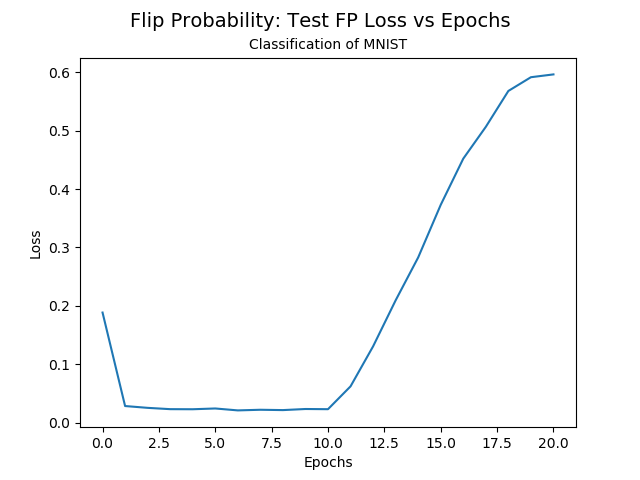
\includegraphics[width=65mm]{figs/run_8/test_losses_fp.png}
    }
    \hspace{0mm}
    \subfloat[third]{
      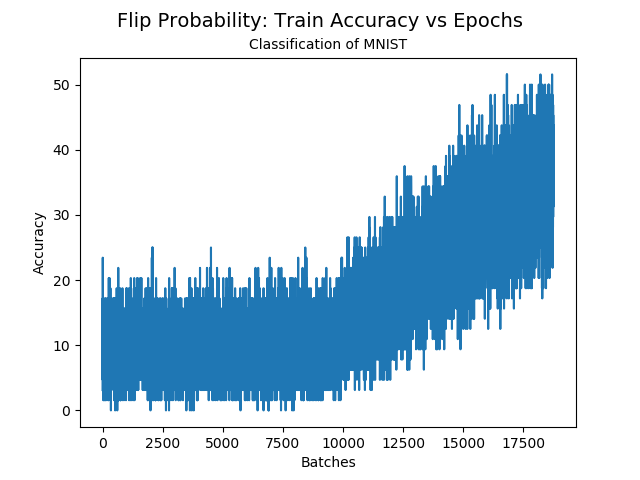
\includegraphics[width=65mm]{figs/run_8/train_accuracy.png}
    }
    \subfloat[forth]{
      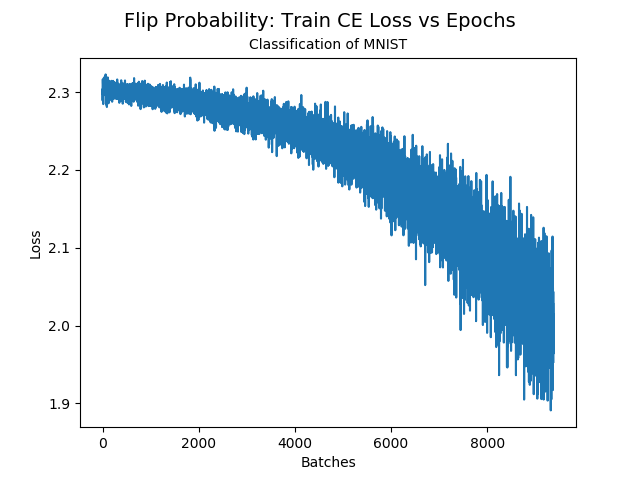
\includegraphics[width=65mm]{figs/run_8/train_losses_ce.png}
    }
    \hspace{0mm}
    \hbox to 67.5mm{}% !!
    \subfloat[fifth]{   % ???
      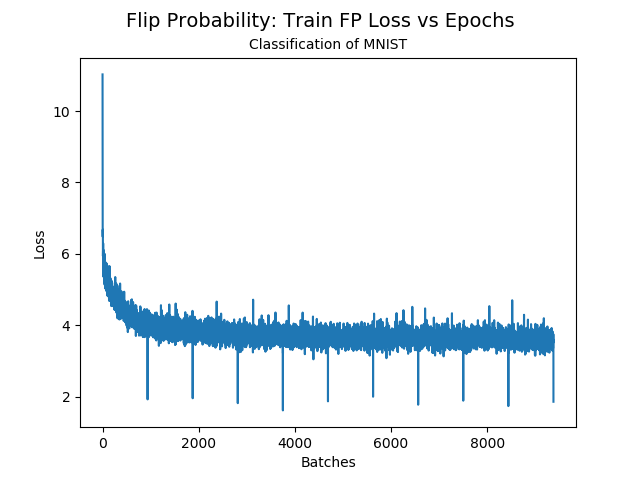
\includegraphics[width=65mm]{figs/run_8/train_losses_fp.png}
    }
    \caption{The results of the eighth training scheme}
    \label{fig:training_scheme_8}
\end{figure}

\begin{figure}[H]
    \centering
    \subfloat[first]{
      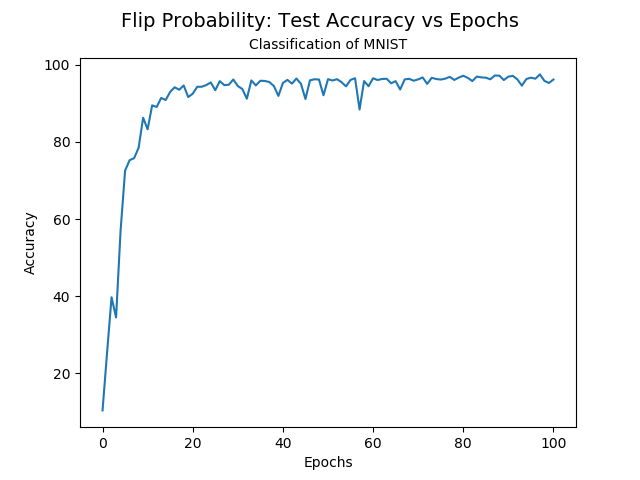
\includegraphics[width=65mm]{figs/run_9/test_accuracy_fp.png}
    }
    \subfloat[second]{
      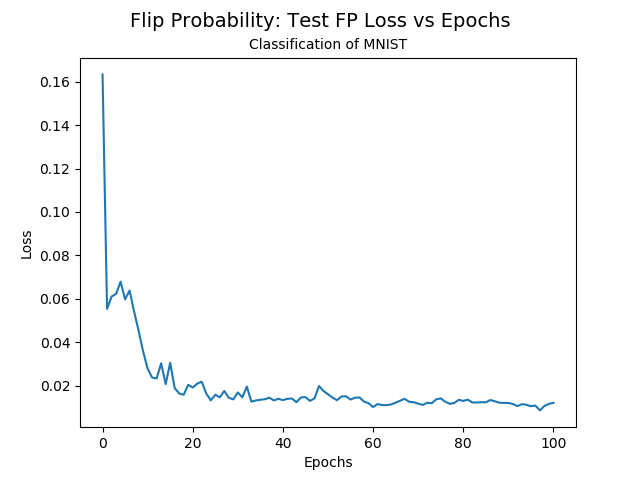
\includegraphics[width=65mm]{figs/run_9/test_losses_fp.png}
    }
    \hspace{0mm}
    \subfloat[third]{
      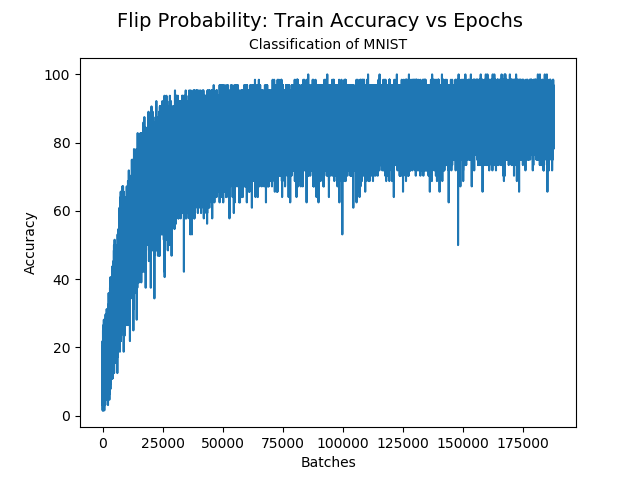
\includegraphics[width=65mm]{figs/run_9/train_accuracy.png}
    }
    \subfloat[forth]{
      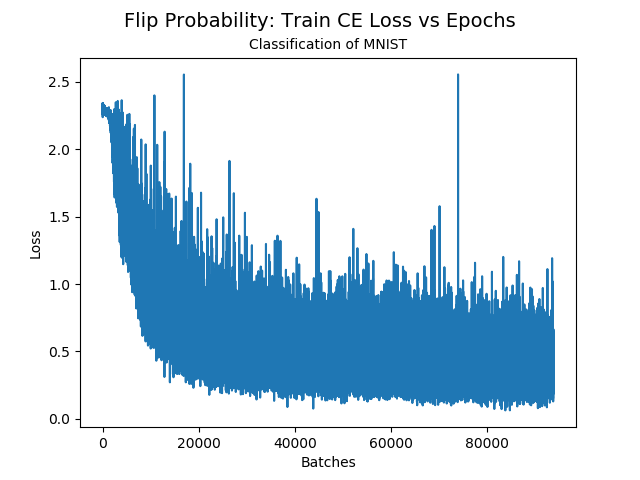
\includegraphics[width=65mm]{figs/run_9/train_losses_ce.png}
    }
    \hspace{0mm}
    \hbox to 67.5mm{}% !!
    \subfloat[fifth]{   % ???
      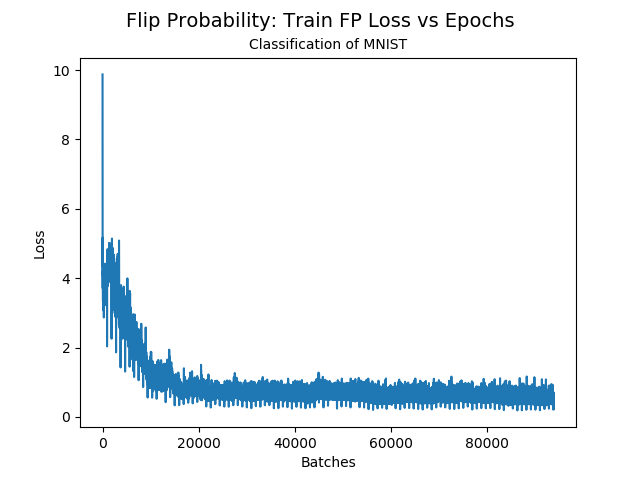
\includegraphics[width=65mm]{figs/run_9/train_losses_fp.png}
    }
    \caption{The results of the ninth training scheme}
    \label{fig:training_scheme_9}
\end{figure}

\begin{figure}[H]
    \centering
    \subfloat[normalised]{
      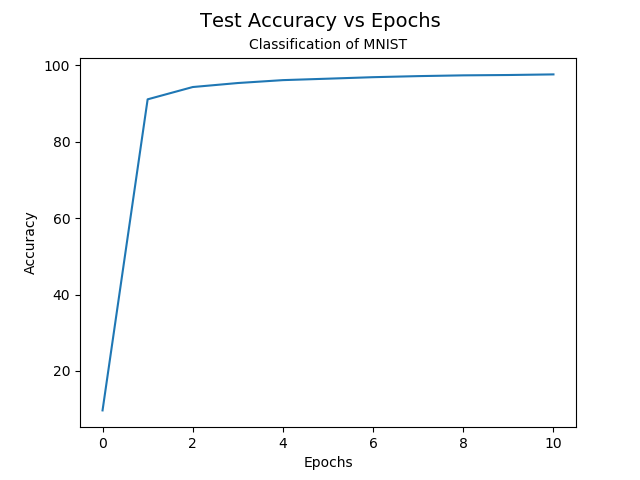
\includegraphics[width=65mm]{figs/run_10/test_accuracy_fp.png}
    }
    \subfloat[normalised]{
      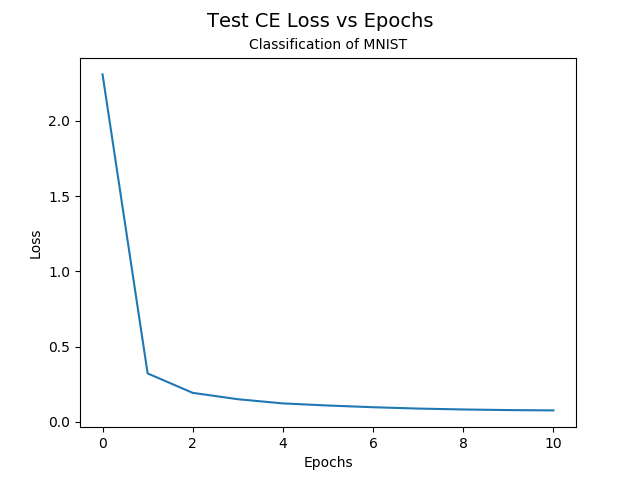
\includegraphics[width=65mm]{figs/run_10/test_losses_fp.png}
    }
    \hspace{0mm}
    \subfloat[normalised]{
      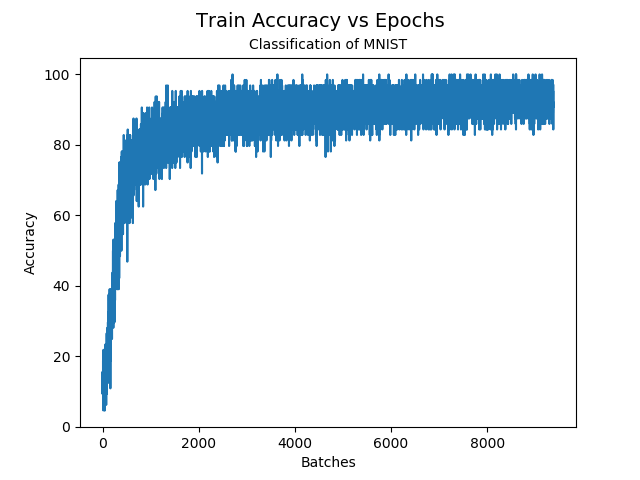
\includegraphics[width=65mm]{figs/run_10/train_accuracy.png}
    }
    \subfloat[normalised]{
      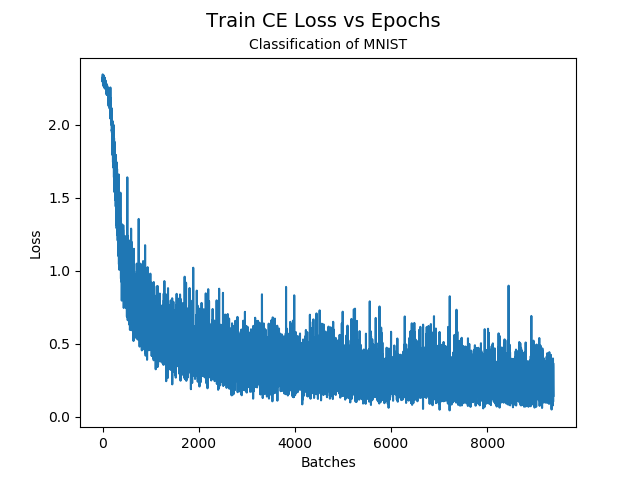
\includegraphics[width=65mm]{figs/run_10/train_losses_ce.png}
    }
    \hspace{0mm}
    \subfloat[no normalisation]{
      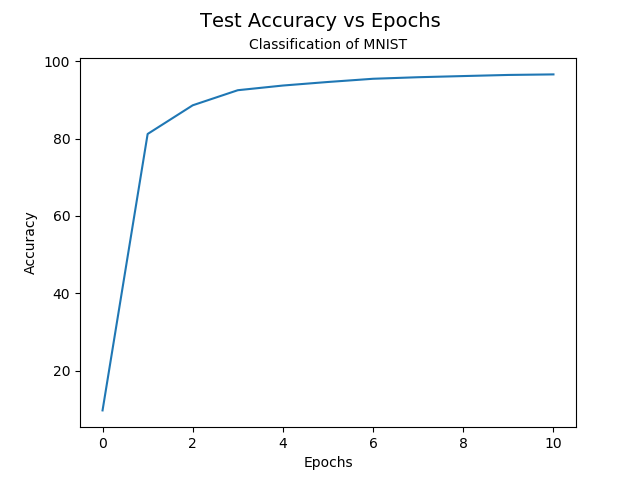
\includegraphics[width=65mm]{figs/run_11/test_accuracy_fp.png}
    }
    \subfloat[no normalisation]{
      \includegraphics[width=65mm]{figs/run_11/test_losses_fp.png}
    }
    \hspace{0mm}
    \subfloat[no normalisation]{
      \includegraphics[width=65mm]{figs/run_11/train_accuracy.png}
    }
    \subfloat[no normalisation]{
      \includegraphics[width=65mm]{figs/run_11/train_losses_ce.png}
    }
    \hspace{0mm}
    
    \caption{The results of the tenth and eleventh training scheme, the baseline scheme, with and without normalisation}
    \label{fig:training_scheme_10_11}
\end{figure}

%\begin{figure}
%\centering
%
%
%\caption{The results of the eleventh training scheme, the baseline with no normalisation}
%\label{fig:training_scheme_11}
%\end{figure}

\begin{figure}[H]
    \centering
    \subfloat[first]{
      \includegraphics[width=65mm]{figs/run_12/test_accuracy_fp.png}
    }
    \subfloat[second]{
      \includegraphics[width=65mm]{figs/run_12/test_losses_fp.png}
    }
    \hspace{0mm}
    \subfloat[third]{
      \includegraphics[width=65mm]{figs/run_12/train_accuracy.png}
    }
    \subfloat[forth]{
      \includegraphics[width=65mm]{figs/run_12/train_losses_ce.png}
    }
    \hspace{0mm}
    \hbox to 67.5mm{}% !!
    \subfloat[fifth]{   % ???
      \includegraphics[width=65mm]{figs/run_12/train_losses_fp.png}
    }
    \caption{The results of the twelfth training scheme}
    \label{fig:training_scheme_12}
\end{figure}

\begin{figure}[H]
    \centering
    \subfloat[first]{
      \includegraphics[width=65mm]{figs/run_13/test_accuracy_fp.png}
    }
    \subfloat[second]{
      \includegraphics[width=65mm]{figs/run_13/test_losses_fp.png}
    }
    \hspace{0mm}
    \subfloat[third]{
      \includegraphics[width=65mm]{figs/run_13/train_accuracy.png}
    }
    \subfloat[forth]{
      \includegraphics[width=65mm]{figs/run_13/train_losses_ce.png}
    }
    \hspace{0mm}
    \hbox to 67.5mm{}% !!
    \subfloat[fifth]{   % ???
      \includegraphics[width=65mm]{figs/run_13/train_losses_fp.png}
    }
    \caption{The results of the thirteenth training scheme}
    \label{fig:training_scheme_13}
\end{figure}

We can see that the baseline schemes, 10/11, clearly achieve a very high accuracy rapidly and without trouble. Removing image normalisation slightly decreases training and testing accuracy during the early stages of training, but otherwise has little effect on the final accuracy.

The third, more refined set of experiments was on the \gls{cifar}-10 data set

The final experiment was an attempt to implement \gls{fp} in a \gls{dl} context, to see if any improvements could be made. We used the Tiny ImageNet data set

\section{Discussion}

Other work leveraging \gls{rp}s exists. For example, \gls{rp}s have been used in projection networks in tandem with the full \gls{nn} to efficiently compress down (reduce the number of parameters) the full networks to lessen the memory footprint. This allows projection networks to run on devices that have resource constraints, such as smartwatches \cite{projection_net}. 


